%!TEX root = main.tex
\begin{figure}[h]
	\caption{No. of attacks on hourly basis}
	\label{fig:A}
	\centering
	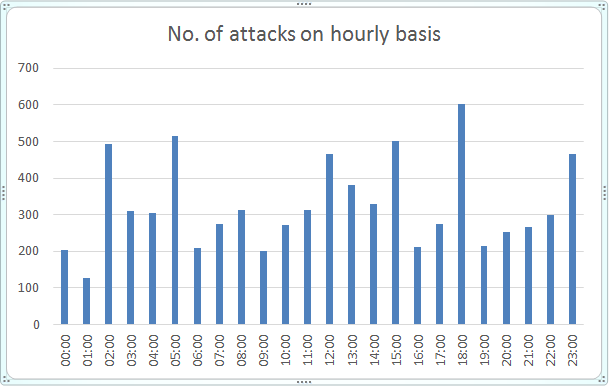
\includegraphics[width=\linewidth]{images/A}
\end{figure}

\begin{figure}[h]
	\caption{No. of attacks during day and night}
	\label{fig:B}
	\centering
	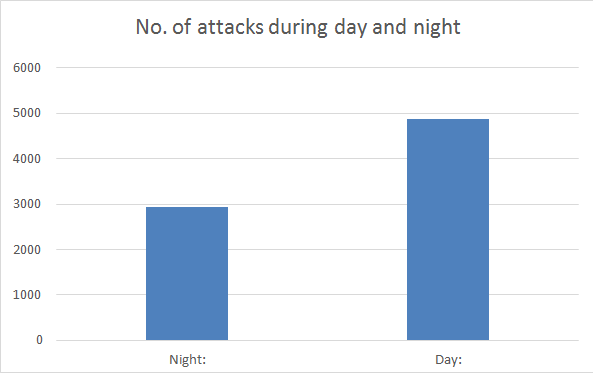
\includegraphics[width=\linewidth]{images/B}
\end{figure}


In figure 4 and 5, we show the no of attacks on hourly basis and no of attacks during day [6 A.M -10 P.M] and night [10 P.M -6 A.M], respectively. From figure 5, we can see significant difference in number of attacks during day and night. We can see 37.5% of the attacks happening during night and 62.5% of the attacks happening during day. This might be due to the fact that infected bots are mostly active (on, working) during day and not active (off, not working) during night. We believe that Botnet infection attempts are higher during the day as a result of this.

\begin{figure}[h]
	\caption{Attacks originating from different countries}
	\label{fig:C}
	\centering
	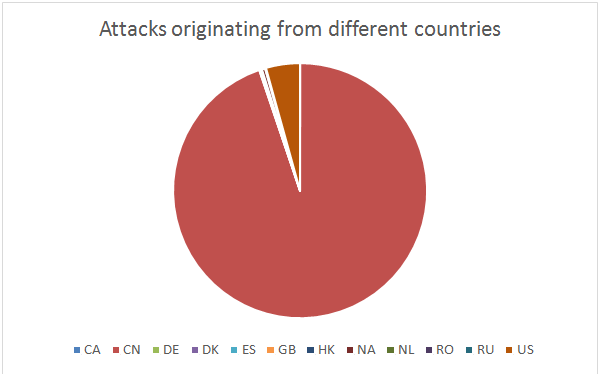
\includegraphics[width=\linewidth]{images/C}
\end{figure}


In figure 6, we show the attacks originating from different countries. The different countries are Canada, China, Denmark, Germany, Hong Kong, NA, Netherlands, Romania, Russia , Spain , U.K and U.S. We have significant no of attacks coming from China which accounts for 94% of attacks. Then we have 4.3% of the attacks originating from U.S and 0.9% of the attacks originating from rest of the countries. We believe that botnet infection attempts are higher in China as Botnets are highly active in China.
